\section{Methods}
\label{sec:Methods}

\subsection{Manufacturing}

\subsubsection{Preparation of reagent}

All reagents were of analytic grade and were used as received from the suppliers without further  purification. Every chemical was bought from Sigma Aldrich, unless stated otherwise. 
Next for facilitation we introduced the formula making use of stoichiometry:

\begin{equation}
\label{eq:RedPrep}
    \frac{m'\cdot v\cdot M}{1000} = m(m',v,M)
\end{equation}


where $m'$ denotes the molecular weight of the reagent, $v$ the desired end-volume of the solution, $M$ the molar concentration and $m$ the needed amount of the substance with unit 'grams', assuming the chemical to be pure. (Example: We want to make 4ml (~$= v$) of solution with \ce{NaOAc} (~$m'_{\ce{NaOAc}}= 82.03 \frac{g}{mol}$) at a concentration of 0.25 M (~$= M$). We now know, that we need to dilute $m \approx 82mg$ \ce{NaOAc} in 4ml of solvent!) 

\paragraph{Gold solution}

We used Gold(III) chloride trihydrate, dissolved in 100 \% ethanol (EtOH). The concentration, unless stated otherwise, was 0.25M and was prepared using the formula (\ref{eq:RedPrep}).


\paragraph{Reduction agent solution}

From the identified reduction agents, the reagent was produced by taking the calculated amount and diluting it in Milli-Q \ce{H2O} until the concentration given was reached. Were the reduction agent was light-sensitive, we put aluminium-foil around the containing reservoir to decrease exposure.

\subsubsection{Sample Fabrication}
\label{subsec:SampleFab}

Define Experiment. We identified 5 independent variables that can be changed.


\begin{multicols}{2}
\begin{itemize}
    \item Gold concentration (\textit{c\textsubscript{gold}})
    \item Gold immersion time (\textit{t\textsubscript{gold}})
    \item Choice of reduction agent
    \item Reduction agent concentration (\textit{c\textsubscript{Red}})
    \item Reduction agent immersion time (\textit{t\textsubscript{Red}})
\end{itemize}
\end{multicols}




\paragraph{Initial Protocol}

\begin{enumerate}
    \item Define which parameters are fixed and which are experimental parameters. Define range you want to investigate.
    
    \item Define concise naming concept, which allows every sample to be uniquely identified.
    
    \item Per sample reserve two petri dishes (PD) and label them in accordance with above mentioned concept. You might add the tag "Pre" and "Post" to existing description. (\textit{PDPre/PDPost}).
    
    \item Put 0.75ml of Gold Solution with \textit{c\textsubscript{gold}} in small, optimally non-translucent viol to account for the light-sensitivity of the gold salt (\textit{Viol}). One viol per sample you wish to investigate. Further decrease of translucency can be achieved by putting aluminium around viol.
    
    \item Put fiber in corresponding \textit{viol} and let immerse according to your defined \textit{t\textsubscript{gold}}.
    \item Take fiber out \textit{viol} and put in \textit{PDPre} to let dry. Note change in colour and/or structure. Experience shows that 30 minutes is sufficient.
    
    \item Gently pour 1ml of reduction agent solution with \textit{c\textsubscript{Red}} over fiber, while making sure the whole fiber is immersed. Note colour gradient in fiber and temporal resolution. Let immerse according to defined \textit{t\textsubscript{Red}}.
    
    \item After passing of time, transfer the fiber gently to \textit{PDPost}, where it will dry.
    \end{enumerate}
    
    \begin{center}
        This marks the end of the fiber fabrication.
    \end{center}


\paragraph{Optimized Protocol} \hfill\newline

1. / 2. are identical to initial protocol.

\begin{enumerate}
\setcounter{enumi}{2}
    
    \item Per sample reserve one petri dish (PD) and one glass slide (GS). Label them in accordance with above mentioned concept, whereas you might add the tag "Pre" to the PD and "Post" to GS description. (\textit{PDPre/GSPost}).
    
    \item Put 0.75ml of Gold Solution with \textit{c\textsubscript{gold}} in small, optimally non-translucent viol to account for the light-sensitivity of the gold salt (\textit{Viol}). One viol per sample you wish to investigate. Further decrease of translucency can be achieved by putting aluminum around viol.
    
    \item Put fiber in corresponding \textit{viol} and let immerse according to your defined \textit{t\textsubscript{gold}}.
    \item Take fiber out viol and put in \textit{PDPre} to let dry. Note change in color and/or structure. Experience shows that 30 minutes is sufficient.
    
    \item Gently pour 1ml of reduction agent solution over fiber, while making sure the whole fiber is immersed. Note color gradient in fiber and temporal resolution. Let immerse according to defined \textit{t\textsubscript{Red}}.
    
    \item After passing of time, transfer the fiber gently to \textit{GSPost}, where it will dry.
    \end{enumerate}
    
    \begin{center}
        This marks the end of the fiber fabrication.
    \end{center}

\subsection{Measurement}

\subsubsection{Preparation}
Prerequisites:
\begin{multicols}{2}
\begin{itemize}
    \item Sample with size $l$
    \item A small piece of paper
    \item 8 Pieces of Tape
    \item Silver Epoxy
    \item Derubberized Cable
\end{itemize}
\end{multicols}

Protocol:

\begin{enumerate}
    \item On piece of paper, put 1 piece of tape (Tape 1) on each side with distance $d < l$ from each other
    \item Now fix both ends of the sample gently without stretching (!) on Tape 1 with another piece of tape (Tape 2).
    \item Then, put free end of cable on end of sample, which is free and over Tape 1. Establish contact and fix cable with Tape 3.
    \item Put Silver Epoxy on sample-cable-interface to facilitate sample-cable-transmission. Bake at 80\textdegree C for 2h. After taking out the oven, put tape 4 perfectly aligned with the medial edge of Tape 1.
\end{enumerate}

    \begin{center}
    \myworries{
    TODO
    Refer to actual figure (Add label, fix picture organisation.)
    TODO}
    
See figure number \ref{fig:MeasPrep} in Appendix for visual description of resistance measurement preparation.
    \end{center}


\subsubsection{Resistance Measurements}

\begin{figure}[H]
    \centerline{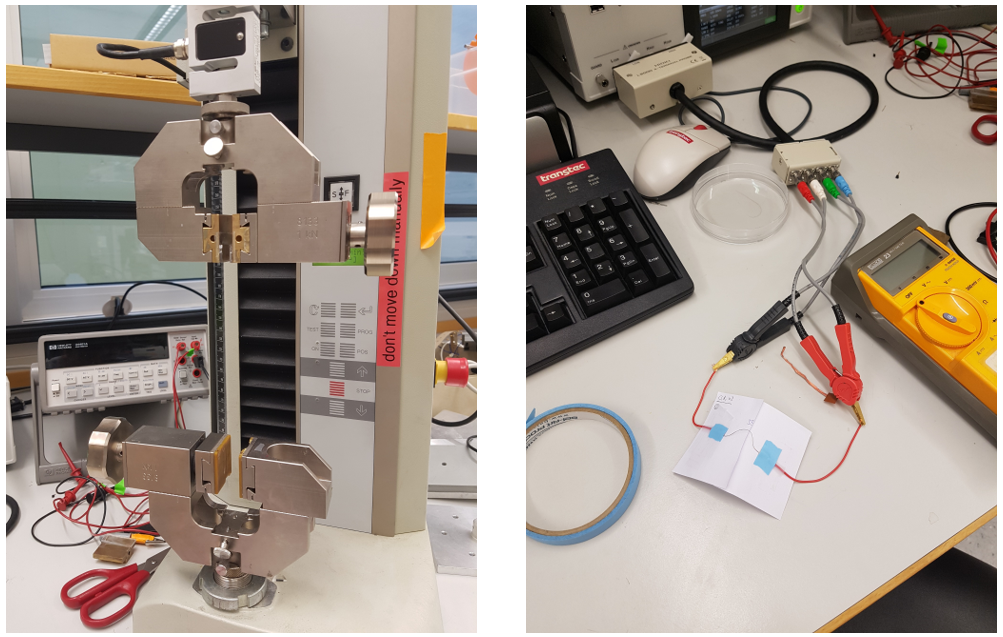
\includegraphics[scale=0.7]{./pic/MethodsResMeasurement.PNG}}
    \caption{Setup of Continuous Resistance Measurement}
    \label{fig:ContResMeas}
\end{figure}

